% ======================= Pre-Amble =========================
      
%Format
\documentclass[11pt, oneside]{article}   	% use "amsart" instead of "article" for AMSLaTeX format 
                     						%imports package {article} and specify option(s) [11pt, oneside]
\usepackage{geometry}                		% See geometry.pdf to learn the layout options. There are lots. 
    \geometry{letterpaper}                   		% ... or a4paper or a5paper or ... 
    %\geometry{landscape}                		% Activate for rotated page geometry

\usepackage[parfill]{parskip}    		        % Activate to begin paragraphs with an empty line rather than an indent

    %Colours
    \usepackage{graphicx, subcaption}
    \usepackage[usenames, dvipsnames]{color}     % font colour:    \textcolor{<colour>}{text}
          									%highlight text:  \colorbox{<color>}{text}
    \usepackage{soul}						%highlight text: \hl{}     %only  yellow								
    									%list of colours: https://www.sharelatex.com/learn/Using_colours_in_LaTeX
    									
    %Bullets
    \usepackage{enumerate}     %specify type of enumeration: \being{enumerate}[<type of enumeration>]
    
    %Footnote Spacing
    \setlength{\footnotesep}{0.4cm}                  %specify spacing b/w footnotes
    \setlength{\skip\footins}{0.6cm}                    % space b/w footnotes and textbody


%Mattematics
    %American Mathematics Society packages
    \usepackage{amsmath}	   %math
    \usepackage{amssymb}       %symbols
    \usepackage{amsthm}          %theorems

    %QED
    \newcommand*{\QEDA}{\hfill\ensuremath{\blacksquare}}         %make qed filled square:    \QEDA
    \newcommand*{\QEDB}{\hfill\ensuremath{\square}}               %make qed empty square: \QEDB 
    
    \renewcommand\qedsymbol{\ensuremath{\blacksquare}}		%Proof environment


%Figures
\usepackage{caption}
\captionsetup[figure]{labelfont=bf}    %make figure labels boldface
\captionsetup[table]{labelfont=bf}     %make table labels boldface

\usepackage[hidelinks]{hyperref}                % Allows for clickable references

    %Tables
    \usepackage[none]{hyphenat}                    % Stops breaking-up words in a table (i.e. no hyphens)                                                             
    
    \usepackage{array}   
        \newcolumntype{x}[1]{>{\centering\let\newline\\\arraybackslash\hspace{0pt}}p{#1}}       %center fixed column width: x{<len>}                      
        \newcolumntype{$}{>{\global\let\currentrowstyle\relax}}                                                   % let us apply things (e.g. bold/italicize) to entire row            
        \newcolumntype{^}{>{\currentrowstyle}}
        \newcommand{\rowstyle}[1]{\gdef\currentrowstyle{#1} #1\ignorespaces}
    
    %Images
    \graphicspath{ {images/} }                          %directory that your images are located in within your current directory
    
    %Diagrams
    \usepackage[latin1]{inputenc}
    \usepackage{tikz}
    	\tikzset{line/.style={-latex'}}
        \usepackage{tkz-berge}
        \usetikzlibrary{shapes,arrows}
        \usetikzlibrary{patterns}			%Specify colours of stuff (e.g. vertices): 
        								%	-> set style: \tikzset{VertexStyle/.append style = {minimum size = 8pt, inner sep = 0pt}} 
								%	-> change individual vertices: \AddVertexColor{white}{1,2} 


%Bibliography
\usepackage[numbers,sort&compress]{natbib}   %for multiple references: sorts  (i.e. [1,2] NOT [2, 1] )
                                           				  %                                     compresses (i.e. [1-3] )
\usepackage[nottoc]{tocbibind}                            %add bibliography to table of contents


%Miscellaneous
\usepackage{dirtytalk}    %quotations: use \say  


%================== Header & Footer =========================
\usepackage{fancyhdr}
\usepackage{lastpage}      %ensures you can reference LastPage (i.e. Page 2 of 10)

\renewcommand{\headrulewidth}{0.4pt}		%Decorative Header line: thickness={0.4pt}
\renewcommand{\footrulewidth}{0.4pt}		%Decorative Footer line: thickness={0.4pt}

\setlength{\headheight}{13.6pt} 		%space b/w top of page & header
\setlength{\headsep}{0.3in}		%space b/w page header and body

%Make Header & Footer    
\pagestyle{fancy}
    \lhead{Stephanie Knill} 		% controls the left corner of the header
    \chead{} 					% controls the center of the header
    \rhead{} 					% controls the right corner of the header
    \lfoot{} 					% controls the left corner of the footer
    \cfoot{Page~\thepage\ of \pageref{LastPage}} 				% controls the center of the footer
    												%Page~\thepage\  if just want Page x
    \rfoot{}			 		% controls the right corner of the footer

% =============================== Document ===================================
\begin{document}

% Title Page
\title{MATH 442 --- Assignment 6 \\
\line(1,0){360} \\              %(slope x, y){length of line}
}
\author{
Stephanie Knill \\
54882113 \\
Due: February 25, 2016}

\date{}                   % Activate:  display a given date (e.g. {August 4} ) or no date (empty {} )
                                    %No activate: display current date
\maketitle

%\thispagestyle{empty}                   %Remove header from this (first) page. Change empty -> plain to keep numbering
%								-> Doesn't matter in this case (b/c title page)
%\cleardoublepage


% ================= Questions ================

\section*{Question 31}

\textbf{Proposition:} Let $G_1$ and $G_2$ be two homeomorphic graphs. Let $G_1$ have $n_1$ vertices and $m_1$ edges, and let $G_2$ have $n_2$ vertices and $m_2$ edges. Show that $m_1 - n_1 = m_2 = n_2$.

\begin{proof}
Let $G_1$ and $G_2$ be two homeomorphic graphs. Let $G_1$ have $n_1$ vertices and $m_1$ edges, and let $G_2$ have $n_2$ vertices and $m_2$ edges. For two graphs to be homeomorphic, we can go between the two graphs by performing one or more of the following operations:
	\begin{enumerate}
		\item Inserting vertices in the middle of an edge
		\item Erasing vertices of degree 2
	\end{enumerate}
	Let us examine the first operation. For $G_2$ of $n_2$ vertices and $m_2$ edges, inserting a vertex will give us a new graph $G_1$ homeomorphic with $n_1$ vertices and $m_1$ edges:
	$$n_1 = n_2 + 1$$
	$$m_1 = m_2 - 1$$
	Taking the difference between $m_1$ and $m_2$, we have
	\begin{align*}
		m_1-n_1 & = (m_2-1)-(n_2+1) \\
		& = m_2-n_2
	\end{align*}
	For the second operation, let us erase a vertex of degree 2 from $G_2$. This will give us a new graph $G_1$ homeomorphic with $n_1$ vertices and $m_1$ edges:
	$$n_1 = n_2 - 1$$
	$$m_1 = m_2 + 1$$
	Taking the difference similarly gives us
	\begin{align*}
		m_1-n_1 & = (m_2+1)-(n_2-1) \\
		& = m_2-n_2
	\end{align*}	
\end{proof}

\section*{Question 32}

\textbf{Proposition:} No polyhedral graph with exactly 30 edges and 11 faces can exist.

\begin{proof}
Assume, to the contrary, that there exists a polyhedral graph with exactly 30 edges and 11 faces. Since a polyhedral graph, by definition, is a simple connected planar graph where each vertex has degree at least 3, we can apply Euler's Theorem to find the number of vertices $v$ of our graph:
\begin{align*}
	v-e+f & =2 \\
	v & = 2 + e -f \\
	& = 2+(30)-(11) \\
	& = 21
\end{align*}
Since each vertex has degree $d_i \geq 3$, we have
\begin{align*}
	3v & \leq 2e
\end{align*}
Substituting $v=21$ and $e=30$ into our inequality
\begin{align*}
	3(21) & \leq 2 (30) \\
	63 & \nleq 60
\end{align*}
we arrive at a contradiction.
\end{proof}


\cleardoublepage
\section*{Question 33}

Let us find the dual of each regular polyhedra
\begin{enumerate}
	\item \textbf{Tetrahedron}
	
	Since the tetrahedron is relatively small (compared to an icosohedron), we can construct the dual graph (Figure \ref{Tetrahedron Dual}) following the two stage algorithm as outlined in \cite{graph}:
	\begin{figure}[h]           
            \centering
              \begin{tikzpicture}[scale=0.75,transform shape]
        		
        		%\GraphInit[vstyle=Classic]					%Make vertice labels outside it
        		\SetVertexNoLabel							%No vertice labels
        		\tikzset{VertexStyle/.append style = {fill=black, circle}}		%Set vertex style        		
			\Vertex [x=0,y=0]{1}
			\Vertex [x=3, y=6]{2}
			\Vertex [x=6, y=0]{3}
			\Vertex [x=3, y=2.5]{4}
		%\SetVertexNoLabel				
        		\tikzset{VertexStyle/.append style = {fill=white, rectangle}}	
			\Vertex [x=3, y=1]{5}
			\Vertex [x=2, y=2.8]{6}
			\Vertex [x=4, y=2.8]{7}
			\Vertex [x=6, y=4]{8}
            
        			\path [thick] (1) edge (2);			%arrows: [line];     label: {$label}$
			\path [thick] (2) edge (3);
			\path [thick] (3) edge (1);
			\path [thick] (1) edge (4);
			\path [thick] (2) edge (4);
			\path [thick] (3) edge (4);
			
			\path [dashed] (5) edge (6);
			\path [dashed] (6) edge (7);
			\path [dashed] (7) edge (5);
			\path [dashed] (7) edge (8);
			\path [dashed] (6) edge [out=120,in=90, bend angle=110, looseness=2.5] (8);
			\path [dashed] (5) edge [out=-80,in=-20, bend angle=110, looseness=2.5] (8);
            	\end{tikzpicture}
            \caption{Graph $G$ and dual graph $G^*$, both of which are isomorphic to a tetrahedron.  $G$ has vertices denoted by black circles and edges by solid lines, and $G^*$ denoted by unfilled squares and edges by dashed lines.}
            \label{Tetrahedron Dual}
        \end{figure}
	
	Alternatively, our tetrahedron graph $G$ has number of edges $e=6$, number of faces $f=4$, and number of vertices $v=4$. For our dual graph $G^*$ with number of edges $e^*$, faces $f^*$, and vertices $v^*$, we have by Lemma 4.12 \cite{graph}
 that 
 \begin{align*}
 	e^* = e \\
	f^* = v \\
	v^*=f
 \end{align*}
	Thus the dual of a tetrahedron has $e^*=6$, $f^*=4$, and $v^*=4$, which is a graph isomorphic to a \textbf{tetrahedron}  (Figure \ref{Tetrahedron}).
	
	\begin{figure}[h]           
            \centering
            \begin{subfigure}[b]{0.45\columnwidth}
            	\centering
             	 \begin{tikzpicture}[scale=0.75,transform shape]
        		
        		%\GraphInit[vstyle=Classic]					%Make vertice labels outside it
        		%\SetVertexNoLabel							%No vertice labels
        		\tikzset{VertexStyle/.append style = {fill=black, circle}}		%Set vertex style        		
			\Vertex [x=0,y=0]{1}
			\Vertex [x=2, y=4]{2}
			\Vertex [x=4, y=0]{3}
			\Vertex [x=2, y=1.5]{4}
        		%\AddVertexColor{white}{1,2} 					%Change individual vertex type
            
        			\path [thick] (1) edge (2);			%arrows: [line];     label: {$label}$
			\path [thick] (2) edge (3);
			\path [thick] (3) edge (1);
			\path [thick] (1) edge (4);
			\path [thick] (2) edge (4);
			\path [thick] (3) edge (4);

            	\end{tikzpicture}
            	\caption{Graph $G$ of a tetrohedron}
            \end{subfigure}
           \begin{subfigure}[b]{0.45\columnwidth}
            	\centering
             	 \begin{tikzpicture}[scale=0.75,transform shape]
        		
        		%\GraphInit[vstyle=Classic]					%Make vertice labels outside it
        		\SetVertexNoLabel							%No vertice labels
        		\tikzset{VertexStyle/.append style = {rectangle}}		%Set vertex style        		
			\Vertex [x=0,y=0]{1}
			\Vertex [x=2, y=4]{2}
			\Vertex [x=4, y=0]{3}
			\Vertex [x=2, y=1.5]{4}
        		%\AddVertexColor{white}{1,2} 					%Change individual vertex type
            
        			\path [dashed] (1) edge (2);			%arrows: [line];     label: {$label}$
			\path [dashed] (2) edge (3);
			\path [dashed] (3) edge (1);
			\path [dashed] (1) edge (4);
			\path [dashed] (2) edge (4);
			\path [dashed] (3) edge (4);

            	\end{tikzpicture}
            	\caption{Dual graph $G^*$ of a tetrohedron}
            \end{subfigure}
           
            \caption{Planar graphs $G$ and $\overline{G}$ of 6 vertices.}
            \label{Tetrahedron}
        \end{figure}
    	
	\item \textbf{Cube}
	
	Our cube graph $G$ has number of edges $e=12$, number of faces $f=6$, and number of vertices $v=8$. For our dual graph $G^*$ with number of edges $e^*$, faces $f^*$, and vertices $v^*$, we have
 that 
 	$$e^* = e = 12$$
	$$f^* = v = 8$$
	$$v^*=f = 6$$
	Thus the dual of a cube is a graph isomorphic to an \textbf{Octahedron}. 
	
	\item \textbf{Octahedron}
	
	By Theorem 4.13 in \cite{graph}, we have that the dual of a dual graph ($G^{**}$) is isomorphic to the original graph ($G^*$). From above, we know that a cube's dual is an octahedron. Thus the dual of an octahedron is a \textbf{Cube}.
	
	\item \textbf{Dodecahedron}
	
	Our dodecahedron graph $G$ has number of edges $e=30$, number of faces $f=20$, and number of vertices $v=12$. For our dual graph $G^*$ with number of edges $e^*$, faces $f^*$, and vertices $v^*$, we have
 that 
 	$$e^* = e = 30$$
	$$f^* = v = 12$$
	$$v^*=f = 20$$
	Thus the dual of a dodecahedron is a graph isomorphic to an \textbf{Icosohedron}. 
	
	\item \textbf{Icosohedron}
	
	Again by Theorem 4.13 in \cite{graph}, we have that the dual of a dual graph ($G^{**}$) is isomorphic to the original graph ($G^*$). From above, we know that a dodecahedron's dual is an icosohedron. Thus the dual of an icosohedron is a \textbf{Dodecahedron}.
	
\end{enumerate}


\section*{Question 34}

\emph{Show the line graph of a tetrahedron graph is the octahedron graph}

Superimposing the line graph $L(G)$ on top of our tetrahedron graph $G$ (Figure \ref{tetra line graph})

\begin{figure}[h]           
            \centering
            \begin{tikzpicture}[scale=0.75,transform shape]
        		
        		%\GraphInit[vstyle=Classic]					%Make vertice labels outside it			
        		\tikzset{VertexStyle/.append style = {fill=white, rectangle}}	
			\Vertex [x=3, y=4]{1}
			\Vertex [x=1.7, y=1.4]{2}
			\Vertex [x=4.3, y=1.4]{3}
			\Vertex [x=1.5, y=3.2]{4}
			\Vertex [x=4.5, y=3.2]{5}
			\Vertex [x=3, y=0]{6}			
		\SetVertexNoLabel							%No vertice labels
        		\tikzset{VertexStyle/.append style = {fill=black, circle}}		%Set vertex style        		
			\Vertex [x=0,y=0]{1t}
			\Vertex [x=3, y=6]{2t}
			\Vertex [x=6, y=0]{3t}
			\Vertex [x=3, y=2.5]{4t}
            
        			\path [thick] (1t) edge (2t);			%arrows: [line];     label: {$label}$
			\path [thick] (2t) edge (3t);
			\path [thick] (3t) edge (1t);
			\path [thick] (1t) edge (4t);
			\path [thick] (2t) edge (4t);
			\path [thick] (3t) edge (4t);
			
			\path [dashed] (1) edge (2);
			\path [dashed] (2) edge (3);
			\path [dashed] (3) edge (1);
			
			\path [dashed] (1) edge (4);
			\path [dashed] (1) edge (5);
			\path [dashed] (2) edge (4);
			\path [dashed] (2) edge (6);
			\path [dashed] (3) edge (5);
			\path [dashed] (3) edge (6);
			
			\path [dashed] (4) edge [out=90,in=90, bend angle=110, looseness=3.5] (5);
			\path [dashed] (4) edge [out=220,in=-135, bend angle=110, looseness=3] (6);
			\path [dashed] (6) edge [out=-45,in=-35, bend angle=110, looseness=3] (5);
            	\end{tikzpicture}
	    	       
            \caption{Graph $G$ of a tetrahedron and its dual graph $G^*$. $G$ has vertices denoted by black circles and edges by solid lines, and $G^*$ denoted by unfilled squares and edges by dashed lines.}
            \label{tetra line graph}
        \end{figure}

	Next, let us separate $L(G)$ from our original graph. Rearranging the orientation of the vertices gives us a graph isomorphic to the octahedron graph (Figure \ref{line graph}).

\begin{figure}[h]           
	\centering
	\begin{tikzpicture}[scale=0.75,transform shape]
        		
        		%\GraphInit[vstyle=Classic]					%Make vertice labels outside it			
        		\tikzset{VertexStyle/.append style = {fill=white, rectangle}}	
			\Vertex [x=3, y=1.2]{1}
			\Vertex [x=2.2, y=3]{2}
			\Vertex [x=3.8, y=3]{3}
			\Vertex [x=0, y=0]{4}
			\Vertex [x=6, y=0]{5}
			\Vertex [x=3, y=6]{6}			
					
			\path [dashed] (1) edge (2);
			\path [dashed] (2) edge (3);
			\path [dashed] (3) edge (1);
			
			\path [dashed] (1) edge (4);
			\path [dashed] (1) edge (5);
			\path [dashed] (2) edge (4);
			\path [dashed] (2) edge (6);
			\path [dashed] (3) edge (5);
			\path [dashed] (3) edge (6);
			
			\path [dashed] (4) edge (6);
			\path [dashed] (4) edge (5);
			\path [dashed] (6) edge (5);			
	  \end{tikzpicture}
	  \caption{Line graph $L(G)$ of a tetrahedron is an octahedron.}
           \label{line graph}
\end{figure}

\emph{Prove that if a simple graph $G$ is regular of degree $k$, then $L(G)$ is regular of degree $2k-2$.}

\begin{proof}
Assume that $G$ is a graph of regular degree $k$. Let us choose any edge $e$ of $G$ which will correspond to a vertex $v^l$ in the line graph $L(G)$. Since each edge connects 2 vertices, we have a total of $2k$ edges meeting at the vertex ends of edge $e$. This means that the vertex $v^l$ is adjacent to $2k$ other vertices in $L(G)$, which gives us a vertex degree of $k^l=2k$. However we have double counted the edge $e$ twice: once for the first vertex end of degree $k$ and a second time for the other vertex of degree $k$. Thus our line graph $L(G)$ has vertices regular of degree $k^l = 2k-2$.
\end{proof}

\section*{Question 35}

\emph{Find two simple graphs $G$ and $H$ such that $G$ and $H$ are \textit{not} isomorphic but $L(G)$ and $L(H)$ are isomorphic.}

Since $L(G)$ is isomorphic to $L(H)$, we have that $e = e^l$. Utilizing proof by inspector gadget, we see that a cycle graph $C_3$ (Figure \ref{graph1}) and a simple connected graph of 4 vertices with one vertex degree 3 and the rest degree 1 (Figure \ref{graph2}) are not isomorphic to each other 

\begin{figure}[h]           
        \centering
        \begin{subfigure}[b]{0.45\columnwidth}
        	\centering
         	\begin{tikzpicture}[scale=0.75,transform shape]
    		
    		%\GraphInit[vstyle=Classic]					%Make vertice labels outside it
    		%\SetVertexNoLabel							%No vertice labels
    		\tikzset{VertexStyle/.append style = {fill=black, circle}}		%Set vertex style        		
			\Vertex [x=0,y=0]{1}
			\Vertex [x=2, y=0]{2}
			\Vertex [x=1, y=2]{3}
    		%\AddVertexColor{white}{1,2} 					%Change individual vertex type
        
    			\path [thick] (1) edge (2);			%arrows: [line];     label: {$label}$
			\path [thick] (2) edge (3);
			\path [thick] (3) edge (1);

        		\end{tikzpicture}
        		\caption{Graph $G$}
		\label{graph1}
       \end{subfigure}
       \begin{subfigure}[b]{0.45\columnwidth}
        	\centering
         	\begin{tikzpicture}[scale=0.75,transform shape]
    		
    		%\GraphInit[vstyle=Classic]					%Make vertice labels outside it
    		%\SetVertexNoLabel							%No vertice labels
    		\tikzset{VertexStyle/.append style = {fill=black, circle}}		%Set vertex style        		
			\Vertex [x=0,y=0]{2}
			\Vertex [x=0, y=2]{1}
			\Vertex [x=2, y=2]{3}
			\Vertex [x=2, y=0]{4}
    		%\AddVertexColor{white}{1,2} 					%Change individual vertex type
        
    			\path [thick] (1) edge (2);			%arrows: [line];     label: {$label}$
			\path [thick] (1) edge (3);
			\path [thick] (1) edge (4);

        		\end{tikzpicture}
        		\caption{Graph $H$}		        
       \label{graph2}
       \end{subfigure}
       \caption{Non-isomorphic graphs $G$ and $H$ with isomorphic line graphs.}
\end{figure}

but whose line graphs are isomorphic (Figure \ref{line graphs}).
\begin{figure}
        	\centering
         \begin{tikzpicture}[scale=0.75,transform shape]
    		
    		%\GraphInit[vstyle=Classic]					%Make vertice labels outside it
    		\SetVertexNoLabel							%No vertice labels
    		\tikzset{VertexStyle/.append style = {fill=white, rectangle}}		%Set vertex style        		
			\Vertex [x=0,y=0]{1}
			\Vertex [x=2, y=0]{2}
			\Vertex [x=1, y=2]{3}
    		%\AddVertexColor{white}{1,2} 					%Change individual vertex type
        
    			\path [dashed] (1) edge (2);			%arrows: [line];     label: {$label}$
			\path [dashed] (2) edge (3);
			\path [dashed] (3) edge (1);

       \end{tikzpicture}
       \caption{Line graphs $L(G)$ and $L(H)$.}		        
       \label{line graphs}
\end{figure}

\section*{Question 36}

\begin{proof}
Let $G$ be a simple graph with vertices $v_1, \ldots , v_n$ of corresponding vertex degree $d_i$ for $1 \leq i \leq n$. To find the total number of edges in $L(G)$, let us first find the number of edges contributed to $L(G)$ for each vertex $v_i$. For a vertex $v_i$ of degree $d_i$, we have $d_i$ edges emerging from it. This means that each of these $d_i$ edges (corresponding to a vertex in the line graph) is adjacent to $d_i - 1$ other edges going into $v_i$. Since there are $d_i$ of these edges, this gives us a total of $d_i(d_i-1)$ edges contributed to $L(G)$ from each vertex $v_i$. However, each edge has been double counted. Thus we only have
$$\frac{d_i(d_i-1)}{2}$$
edges contributed per vertex $v_i$. Summating over all vertices $v_1, \ldots, v_n$ gives us the total number of edges in $L(G)$ to be
$$\sum_{i=1}^n \frac{d_i(d_i-1)}{2}$$
\end{proof}


% =========================== Bibliography ==========================

\cleardoublepage

% Method 1
\begin{thebibliography}{10}

\bibitem{graph} Wilson, Robin J. (2010). \textit{Introduction to Graph Theory} (5th ed.). Harlow, England: Pearson Education Limited.
%reference this: \cite{graph}

\end{thebibliography}
\end{document} 